\chapter{À l'intérieur de l'atome}\label{ch:g9:inside-the-atom}

En 1909, dans un laboratoire de Manchester, on bombarda une feuille d'or
épaisse de quelques centaines d'\omterm{def:g7:atoms-and-molecules:atom}{atomes} avec un faisceau de minuscules
particules rapides. Presque toutes la traversèrent tout droit, comme si
l'or était vide. Mais environ une sur plusieurs milliers rebondit en
arrière. «~C'était comme si l'on tirait un obus de quinze pouces sur une
feuille de papier de soie et qu'il revenait vous frapper~», dit Ernest
Rutherford, dont les élèves avaient réalisé l'expérience. L'\omterm{def:g7:atoms-and-molecules:atom}{atome}, le
morceau de matière insécable, avait une structure --- et il était
presque entièrement vide.

\begin{recall}
Toute la matière est faite d'\omterm{def:g7:atoms-and-molecules:atom}{atomes}, d'une centaine de sortes
différentes, chacune ayant un symbole comme \ce{H}, \ce{C}, \ce{O},
\ce{Fe}. Les \omterm{def:g7:atoms-and-molecules:atom}{atomes} s'assemblent en \omterm{def:g7:atoms-and-molecules:molecule}{molécules}, décrites par des formules
comme \ce{H2O} (\cref{ch:g7:atoms-and-molecules}).
\end{recall}

\section{Noyau et électrons}

\begin{definition}[Noyau et électron]\label{def:g9:inside-the-atom:nucleus}
Tout \omterm{def:g7:atoms-and-molecules:atom}{atome} possède un cœur minuscule et lourd, le
\emph{noyau}\index{noyau}, qui porte une charge électrique positive.
Autour de lui se déplacent des particules beaucoup plus légères, les
\emph{électrons}\index{electron@électron}, qui portent chacun la même charge
négative, $-e$.
\end{definition}

\begin{proposition}[Un atome est neutre]\label{prop:g9:inside-the-atom:neutral}
% ledger: const:e
Un \omterm{def:g7:atoms-and-molecules:atom}{atome}, dans son ensemble, ne porte aucune charge électrique~: la
charge positive de son \omterm{def:g9:inside-the-atom:nucleus}{noyau} est exactement compensée par les charges
négatives de ses \omterm{def:g9:inside-the-atom:nucleus}{électrons}. La charge $e$ est minuscule~:
$e = \qty{1.60e-19}{C}$ (le coulomb, unité de charge, relève du livre de
physique).
\end{proposition}

\begin{omfigure}
\begin{tikzpicture}[font=\small]
  \shade[inner color=omDef!35, outer color=white] (0,0) circle (2.2);
  \draw[omDef!60, dashed] (0,0) circle (2.2);
  \foreach \a/\r in {20/1.6,95/1.1,150/1.9,215/1.4,290/1.7,340/0.9} {
    \fill[omDef] (\a:\r) circle (0.06);
    \node[font=\scriptsize, omDef] at ($(\a:\r)+(0.18,0.16)$) {$-$};
  }
  \fill[red!70!black] (0,0) circle (0.1);
  \draw[<-, omProp, thick] (-0.12,0.02) -- (-3.0,0.9) node[left, text=black, align=right]
    {noyau~: minuscule,\\ lourd, positif};
  \draw[<-, omProp, thick] ($(20:1.6)+(0.08,0.02)$) -- (3.0,0.9) node[right, text=black]
    {un électron~: léger, négatif};
  \draw[<-, omProp, thick] (300:2.2) -- (3.0,-1.4) node[right, text=black, align=left]
    {les électrons se déplacent en un nuage\\ autour du noyau};
\end{tikzpicture}

{\small Un \omterm{def:g7:atoms-and-molecules:atom}{atome}, sans respect de l'échelle. Si le \omterm{def:g9:inside-the-atom:nucleus}{noyau} était dessiné de
la taille du point rouge, le nuage d'\omterm{def:g9:inside-the-atom:nucleus}{électrons} mesurerait quelques
centaines de mètres.}
\end{omfigure}

\section{Protons et neutrons}

\begin{definition}[Proton, neutron, nucléon]\label{def:g9:inside-the-atom:proton}
Le \omterm{def:g9:inside-the-atom:nucleus}{noyau} est formé de deux sortes de particules~: les
\emph{protons}\index{proton}, qui portent chacun la charge $+e$, et les
\emph{neutrons}\index{neutron}, qui ne portent pas de charge. Protons et
neutrons, qui ont presque la même masse, sont appelés ensemble
\emph{nucléons}\index{nucleon@nucléon}.
\end{definition}

\begin{definition}[Numéro atomique et nombre de masse]\label{def:g9:inside-the-atom:atomic-number}
Le nombre de \omterm{def:g9:inside-the-atom:proton}{protons} d'un \omterm{def:g9:inside-the-atom:nucleus}{noyau} est le \emph{numéro
atomique}\index{numero atomique@numéro atomique}, noté $Z$. Le nombre de \omterm{def:g9:inside-the-atom:proton}{nucléons}
(\omterm{def:g9:inside-the-atom:proton}{protons} et \omterm{def:g9:inside-the-atom:proton}{neutrons} ensemble) est le \emph{nombre de masse}\index{nombre de masse},
noté $A$. Le nombre de \omterm{def:g9:inside-the-atom:proton}{neutrons} est $N = A - Z$.
\end{definition}

\begin{notation}[L'écriture conventionnelle du noyau]\label{not:g9:inside-the-atom:symbol}
Un \omterm{def:g7:atoms-and-molecules:atom}{atome} dont le \omterm{def:g9:inside-the-atom:nucleus}{noyau} est donné s'écrit avec son symbole, le \omterm{def:g9:inside-the-atom:atomic-number}{nombre de
masse} en haut à gauche et le \omterm{def:g9:inside-the-atom:atomic-number}{numéro atomique} en bas à gauche~:
\ce{^{A}_{Z}X}. Par exemple, \ce{^{12}_{6}C} a 6 \omterm{def:g9:inside-the-atom:proton}{protons} et $12 - 6 =
6$ \omterm{def:g9:inside-the-atom:proton}{neutrons}~; \ce{^{56}_{26}Fe} a 26 \omterm{def:g9:inside-the-atom:proton}{protons} et 30 \omterm{def:g9:inside-the-atom:proton}{neutrons}.
\end{notation}

\begin{method}[Lire l'écriture conventionnelle d'un noyau]\label{met:g9:inside-the-atom:read}
Pour \ce{^{A}_{Z}X}~:
\begin{enumerate}
  \item \omterm{def:g9:inside-the-atom:proton}{protons}~: $Z$~;
  \item \omterm{def:g9:inside-the-atom:proton}{neutrons}~: $A - Z$~;
  \item \omterm{def:g9:inside-the-atom:nucleus}{électrons} de l'\omterm{def:g7:atoms-and-molecules:atom}{atome} neutre~: $Z$, autant que de \omterm{def:g9:inside-the-atom:proton}{protons}.
\end{enumerate}
Pour \ce{^{23}_{11}Na}~: 11 \omterm{def:g9:inside-the-atom:proton}{protons}, 12 \omterm{def:g9:inside-the-atom:proton}{neutrons}, 11 \omterm{def:g9:inside-the-atom:nucleus}{électrons}.
\end{method}

\begin{omfigure}
\begin{tikzpicture}[font=\small]
  \node[font=\Huge, inner sep=1pt] (x) at (0,0) {\ce{^{35}_{17}Cl}};
  \draw[<-, omProp, thick, shorten <=3pt] ([xshift=5pt,yshift=-7pt]x.north west) -- (-2.6,1.0)
    node[left, text=black, align=right] {nombre de masse $A = 35$~:\\ protons + neutrons};
  \draw[<-, omProp, thick, shorten <=3pt] ([xshift=5pt,yshift=7pt]x.south west) -- (-2.6,-1.0)
    node[left, text=black, align=right] {numéro atomique $Z = 17$~:\\ protons};
  \draw[<-, omProp, thick] ([xshift=2pt]x.east) -- (2.2,0) node[right, text=black,
    align=left] {symbole de l'élément~:\\ le chlore};
\end{tikzpicture}

{\small Lire l'écriture conventionnelle d'un \omterm{def:g9:inside-the-atom:nucleus}{noyau}~: cet \omterm{def:g7:atoms-and-molecules:atom}{atome} de chlore
a 17 \omterm{def:g9:inside-the-atom:proton}{protons}, $35 - 17 = 18$ \omterm{def:g9:inside-the-atom:proton}{neutrons}, et 17 \omterm{def:g9:inside-the-atom:nucleus}{électrons} quand il est
neutre.}
\end{omfigure}

\section{L'élément chimique et ses isotopes}

\begin{definition}[Élément chimique]\label{def:g9:inside-the-atom:element}
Un \emph{élément chimique}\index{element chimique@élément chimique} est l'ensemble de tous
les \omterm{def:g7:atoms-and-molecules:atom}{atomes}, et de tous les \omterm{def:g7:atoms-and-molecules:atom}{atomes} chargés qui en dérivent, qui ont le
même \omterm{def:g9:inside-the-atom:atomic-number}{numéro atomique} $Z$. Chaque élément a un nom et un symbole~: tout
\omterm{def:g7:atoms-and-molecules:atom}{atome} possédant 6 \omterm{def:g9:inside-the-atom:proton}{protons} est un \omterm{def:g7:atoms-and-molecules:atom}{atome} de carbone, \ce{C}~; tout \omterm{def:g7:atoms-and-molecules:atom}{atome}
possédant 8 \omterm{def:g9:inside-the-atom:proton}{protons} est un \omterm{def:g7:atoms-and-molecules:atom}{atome} d'oxygène, \ce{O}.
\end{definition}

\begin{definition}[Isotopes]\label{def:g9:inside-the-atom:isotope}
Des \omterm{def:g7:atoms-and-molecules:atom}{atomes} d'un même élément qui ont des nombres de \omterm{def:g9:inside-the-atom:proton}{neutrons} différents,
et donc des \omterm{def:g9:inside-the-atom:atomic-number}{nombres de masse} différents, sont des
\emph{isotopes}\index{isotope} de cet élément. Ils ont le même $Z$ et
des $A$ différents.
\end{definition}

\begin{example}[Isotopes du carbone et de l'hydrogène]\label{ex:g9:inside-the-atom:isotopes}
% ledger: iso:C12, iso:C13, iso:H2
Le carbone naturel contient environ \qty{98.9}{\percent} de carbone~12,
\ce{^{12}_{6}C}, et \qty{1.1}{\percent} de carbone~13, \ce{^{13}_{6}C},
avec une trace de carbone~14, \ce{^{14}_{6}C}, dont la lente
transformation en un autre \omterm{def:g9:inside-the-atom:nucleus}{noyau} sert à dater le bois et les os anciens
(la radioactivité relève du livre de physique). L'hydrogène a trois
\omterm{def:g9:inside-the-atom:isotope}{isotopes}~: \ce{^{1}_{1}H}, sans aucun \omterm{def:g9:inside-the-atom:proton}{neutron}, de loin le plus courant~;
le deutérium \ce{^{2}_{1}H}, quelques \omterm{def:g7:atoms-and-molecules:atom}{atomes} sur cent mille~; et le
tritium \ce{^{3}_{1}H}.
\end{example}

\begin{proposition}[Les isotopes ont la même chimie]\label{prop:g9:inside-the-atom:alike}
La chimie d'un \omterm{def:g7:atoms-and-molecules:atom}{atome} dépend de ses \omterm{def:g9:inside-the-atom:nucleus}{électrons}, et les \omterm{def:g9:inside-the-atom:isotope}{isotopes} d'un
élément ont le même nombre d'\omterm{def:g9:inside-the-atom:nucleus}{électrons}. Les \omterm{def:g9:inside-the-atom:isotope}{isotopes} réagissent donc de
la même façon~: l'eau fabriquée avec du deutérium a presque exactement
l'aspect et le comportement de l'eau ordinaire.
\end{proposition}

\begin{omfigure}
\begin{tikzpicture}[font=\small, p/.style={circle, inner sep=0pt, minimum size=4.2mm,
    ball color=red!65}, n/.style={circle, inner sep=0pt, minimum size=4.2mm,
    ball color=black!20}]
  \node[p] at (0,0) {};
  \node[anchor=north, align=center] at (0,-0.45) {\ce{^{1}_{1}H}\\ 1 proton};
  \node[p] at (3.0,0) {}; \node[n] at (3.35,0.1) {};
  \node[anchor=north, align=center] at (3.2,-0.45) {\ce{^{2}_{1}H}\\ 1 proton, 1 neutron};
  \node[p] at (6.4,0) {}; \node[n] at (6.75,0.12) {}; \node[n] at (6.55,0.35) {};
  \node[anchor=north, align=center] at (6.6,-0.45) {\ce{^{3}_{1}H}\\ 1 proton, 2 neutrons};
  \node[draw=black!30, fill=red!65, circle, minimum size=3mm, inner sep=0pt] at (9.1,0.2) {};
  \node[anchor=west] at (9.3,0.2) {proton};
  \node[draw=black!30, fill=black!20, circle, minimum size=3mm, inner sep=0pt] at (9.1,-0.3) {};
  \node[anchor=west] at (9.3,-0.3) {neutron};
\end{tikzpicture}

{\small Les noyaux des trois \omterm{def:g9:inside-the-atom:isotope}{isotopes} de l'hydrogène~: un \omterm{def:g9:inside-the-atom:proton}{proton}
chacun, et 0, 1 ou 2 \omterm{def:g9:inside-the-atom:proton}{neutrons}.}
\end{omfigure}

\section{Tailles et masses}

\begin{proposition}[Le noyau est minuscule et contient presque toute la masse]\label{prop:g9:inside-the-atom:sizes}
% ledger: const:a0, r:proton, const:mp, const:mn, const:me
Un \omterm{def:g7:atoms-and-molecules:atom}{atome} mesure environ \qty{e-10}{m}~; son \omterm{def:g9:inside-the-atom:nucleus}{noyau}, de \qty{e-15}{m} à
\qty{e-14}{m}~: il est dix mille à cent mille fois plus petit. Les masses
des particules sont
\[
  m_p = \qty{1.673e-27}{kg},\qquad m_n = \qty{1.675e-27}{kg},\qquad
  m_e = \qty{9.11e-31}{kg}.
\]
Un \omterm{def:g9:inside-the-atom:proton}{proton} est environ 1836 fois plus lourd qu'un \omterm{def:g9:inside-the-atom:nucleus}{électron}~: plus de
\qty{99.9}{\percent} de la masse d'un \omterm{def:g7:atoms-and-molecules:atom}{atome} se trouve donc dans son
\omterm{def:g9:inside-the-atom:nucleus}{noyau}.
\end{proposition}

\begin{example}[Une bille dans un stade]\label{ex:g9:inside-the-atom:marble}
Si le \omterm{def:g9:inside-the-atom:nucleus}{noyau} d'un \omterm{def:g7:atoms-and-molecules:atom}{atome} était une bille de \qty{1}{cm}, l'\omterm{def:g7:atoms-and-molecules:atom}{atome}
mesurerait environ $\qty{1}{cm} \times 100\,000 = \qty{1}{km}$~: une
bille au milieu d'un immense stade, avec quelques grains de poussière
--- les \omterm{def:g9:inside-the-atom:nucleus}{électrons} --- qui tourbillonnent autour des tribunes. La matière
est surtout faite de vide.
\end{example}

\begin{method}[La masse d'un atome]\label{met:g9:inside-the-atom:mass}
Comme les \omterm{def:g9:inside-the-atom:proton}{protons} et les \omterm{def:g9:inside-the-atom:proton}{neutrons} ont presque la même masse et que les
\omterm{def:g9:inside-the-atom:nucleus}{électrons} sont très légers, la masse d'un \omterm{def:g7:atoms-and-molecules:atom}{atome} est proche de $A \times
\qty{1.67e-27}{kg}$, où $A$ est son \omterm{def:g9:inside-the-atom:atomic-number}{nombre de masse}. Un \omterm{def:g7:atoms-and-molecules:atom}{atome} de
carbone~12~: $12 \times 1.67 \times 10^{-27} = \qty{2.00e-26}{kg}$.
\end{method}

\section{Une brève histoire du modèle de l'atome}

\begin{history}[De l'insécable au noyau, 1897--1932]
En 1897, J.~J.~Thomson découvrit l'\omterm{def:g9:inside-the-atom:nucleus}{électron}, une particule bien plus
légère que n'importe quel \omterm{def:g7:atoms-and-molecules:atom}{atome}~: on pouvait donc couper les \omterm{def:g7:atoms-and-molecules:atom}{atomes}. Il
se représenta l'\omterm{def:g7:atoms-and-molecules:atom}{atome} comme une boule de matière positive parsemée
d'\omterm{def:g9:inside-the-atom:nucleus}{électrons}. En 1909--1911, l'expérience de la feuille d'or de l'équipe
de Rutherford montra que la charge positive et presque toute la masse
se trouvent dans un \omterm{def:g9:inside-the-atom:nucleus}{noyau} minuscule. En 1913, Niels Bohr proposa que les
\omterm{def:g9:inside-the-atom:nucleus}{électrons} occupent des niveaux d'énergie fixes autour de lui, et en
1932 James Chadwick découvrit le \omterm{def:g9:inside-the-atom:proton}{neutron}.
\end{history}

\begin{omfigure}
\begin{minipage}[b]{0.3\linewidth}\centering
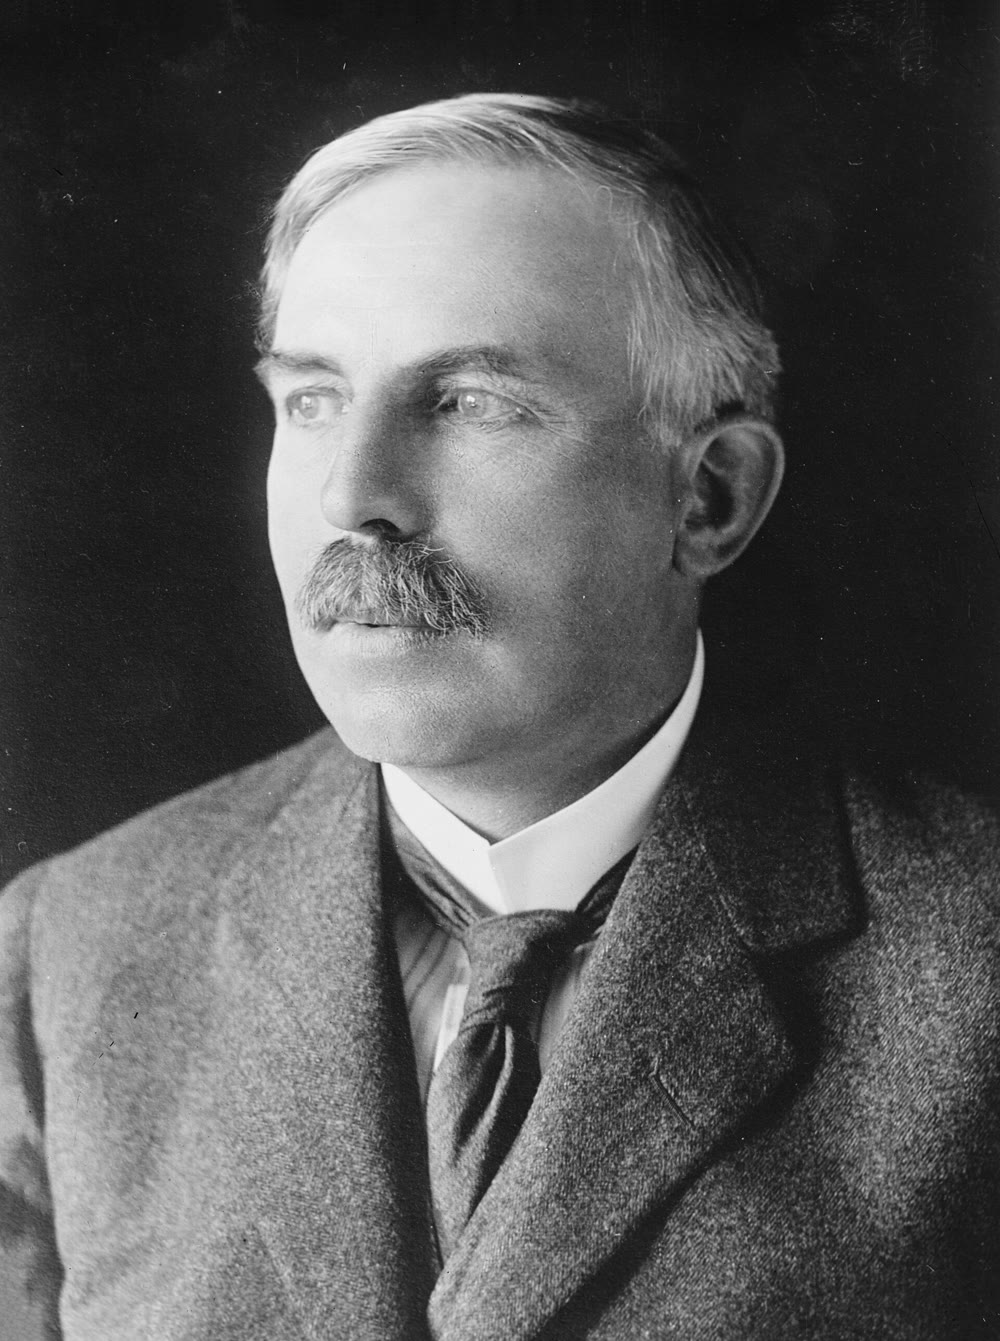
\includegraphics[width=\linewidth]{images/book1/rutherford.jpg}

{\small Ernest Rutherford (1871--1937).}
\end{minipage}\hfill
\begin{minipage}[b]{0.66\linewidth}\centering
\begin{tikzpicture}[font=\small]
  \fill[black!45] (0,-0.5) rectangle (0.9,0.5);
  \node[anchor=north, align=center] at (0.45,-0.55) {source de\\ particules alpha};
  \draw[->, thick, red!70!black] (0.9,0) -- (2.8,0);
  \fill[yellow!70!orange] (2.8,-1.6) rectangle (2.88,1.6);
  \node[anchor=north] at (2.84,-1.65) {feuille d'or};
  \draw[omDef!40, line width=4pt] (5.6,-1.8) arc[start angle=-30, end angle=30, radius=3.6];
  \foreach \y in {-0.3,-0.1,0.1,0.3} \draw[->, red!70!black] (2.88,\y) -- (5.3,\y);
  \draw[->, red!70!black] (2.88,0.05) -- (5.0,1.15);
  \draw[->, red!70!black] (2.88,-0.05) -- (4.9,-1.3);
  \draw[->, red!70!black, thick] (2.8,0.02) .. controls (2.2,0.35) .. (1.6,0.95);
  \node[anchor=west, align=left, font=\footnotesize] at (6.25,0) {la plupart\\ traversent\\ tout droit};
  \node[anchor=south, align=center, font=\footnotesize] at (1.6,1.0) {de très rares\\ rebondissent};
\end{tikzpicture}

{\small L'expérience de la feuille d'or~: la plupart des particules la
traversent tout droit~; quelques-unes sont déviées~; de très rares
rebondissent sur un \omterm{def:g9:inside-the-atom:nucleus}{noyau}.}
\end{minipage}
\end{omfigure}

\section{Exercices}

\begin{exercise}[$\star$]\label{exo:g9:inside-the-atom:1}
Nomme les particules du \omterm{def:g9:inside-the-atom:nucleus}{noyau} et les particules qui l'entourent, avec le
signe de leur charge.
\end{exercise}

\begin{exercise}[$\star$]\label{exo:g9:inside-the-atom:2}
Donne le nombre de \omterm{def:g9:inside-the-atom:proton}{protons}, de \omterm{def:g9:inside-the-atom:proton}{neutrons} et d'\omterm{def:g9:inside-the-atom:nucleus}{électrons} de
\ce{^{16}_{8}O}, \ce{^{27}_{13}Al} et \ce{^{40}_{20}Ca}.
\end{exercise}

\begin{exercise}[$\star$]\label{exo:g9:inside-the-atom:3}
Pourquoi un \omterm{def:g7:atoms-and-molecules:atom}{atome} est-il électriquement neutre~?
\end{exercise}

\begin{exercise}[$\star$]\label{exo:g9:inside-the-atom:4}
Un \omterm{def:g7:atoms-and-molecules:atom}{atome} possède 26 \omterm{def:g9:inside-the-atom:proton}{protons} et 30 \omterm{def:g9:inside-the-atom:proton}{neutrons}. Écris l'écriture
conventionnelle de son \omterm{def:g9:inside-the-atom:nucleus}{noyau} (l'élément est le fer, \ce{Fe}).
\end{exercise}

\begin{exercise}[$\star\star$]\label{exo:g9:inside-the-atom:5}
\ce{^{35}_{17}Cl} et \ce{^{37}_{17}Cl} sont-ils le même élément~?
Sont-ils \omterm{def:g9:inside-the-atom:isotope}{isotopes}~? Explique.
\end{exercise}

\begin{exercise}[$\star\star$]\label{exo:g9:inside-the-atom:6}
\ce{^{14}_{6}C} et \ce{^{14}_{7}N} sont-ils \omterm{def:g9:inside-the-atom:isotope}{isotopes}~? Explique.
\end{exercise}

\begin{exercise}[$\star\star$]\label{exo:g9:inside-the-atom:7}
Calcule, en écriture scientifique, la masse approchée d'un \omterm{def:g7:atoms-and-molecules:atom}{atome} de
\ce{^{56}_{26}Fe}.
\end{exercise}

\begin{exercise}[$\star\star$]\label{exo:g9:inside-the-atom:8}
Dans l'expérience de la feuille d'or, pourquoi la plupart des
particules traversent-elles l'or tout droit~?
\end{exercise}

\begin{exercise}[$\star\star$]\label{exo:g9:inside-the-atom:9}
Combien de fois un \omterm{def:g9:inside-the-atom:nucleus}{noyau} de \qty{e-15}{m} est-il plus petit qu'un \omterm{def:g7:atoms-and-molecules:atom}{atome}
(\qty{e-10}{m})~? Écris la réponse sous forme d'une puissance de dix.
\end{exercise}

\begin{exercise}[$\star\star$]\label{exo:g9:inside-the-atom:10}
Pourquoi les \omterm{def:g9:inside-the-atom:isotope}{isotopes} d'un élément ont-ils la même chimie~?
\end{exercise}

\begin{exercise}[$\star\star\star$]\label{exo:g9:inside-the-atom:11}
Un \omterm{def:g7:atoms-and-molecules:atom}{atome} de fer possède 26 \omterm{def:g9:inside-the-atom:nucleus}{électrons}. Calcule leur masse totale, puis
la fraction de la masse d'un \omterm{def:g7:atoms-and-molecules:atom}{atome} de \ce{^{56}_{26}Fe} qu'ils
représentent (utilise la masse trouvée à l'exercice~7).
\end{exercise}

\begin{exercise}[$\star\star\star$]\label{exo:g9:inside-the-atom:12}
% ledger: iso:Cu63, iso:Cu65
Le cuivre naturel contient \qty{69.15}{\percent} de cuivre~63 et
\qty{30.85}{\percent} de cuivre~65. Sur 10\,000 \omterm{def:g7:atoms-and-molecules:atom}{atomes} de cuivre,
combien y en a-t-il de chaque \omterm{def:g9:inside-the-atom:isotope}{isotope}~? Quel est le nombre moyen de
\omterm{def:g9:inside-the-atom:proton}{nucléons} par \omterm{def:g7:atoms-and-molecules:atom}{atome} de cuivre~?
\end{exercise}

\clearpage % garde le titre avec l'encadré de son problème (il était resté seul en bas de page)
\section{Problème~: peser le chlore}

\begin{problem}[{Problème du week-end --- deux isotopes du chlore, la masse
de chaque atome, et la masse moyenne d'un atome de chlore}]
\label{pb:g9:inside-the-atom:1}
% ledger: iso:Cl35, iso:Cl37, const:me, const:mp, const:mn
Le chlore naturel est un \omterm{def:g6:pure-substances-and-mixtures:mixture}{mélange} de deux \omterm{def:g9:inside-the-atom:isotope}{isotopes}, le chlore~35 et le
chlore~37~: sur 1000 \omterm{def:g7:atoms-and-molecules:atom}{atomes} de chlore, environ 758 sont du chlore~35 et
242 du chlore~37. On prendra pour masse d'un \omterm{def:g9:inside-the-atom:proton}{nucléon} \qty{1.67e-27}{kg}
et pour masse d'un \omterm{def:g9:inside-the-atom:nucleus}{électron} \qty{9.11e-31}{kg}. Le \omterm{def:g9:inside-the-atom:atomic-number}{numéro atomique} du
chlore est 17.

\medskip
\noindent\textbf{Partie I --- Deux noyaux.}
\begin{enumerate}
  \item Écris l'écriture conventionnelle des noyaux des deux \omterm{def:g9:inside-the-atom:isotope}{isotopes}.
  \item Donne le nombre de \omterm{def:g9:inside-the-atom:proton}{protons}, de \omterm{def:g9:inside-the-atom:proton}{neutrons} et d'\omterm{def:g9:inside-the-atom:nucleus}{électrons} de chacun.
  \item Pourquoi les appelle-t-on tous deux chlore~? Pourquoi sont-ils
        \omterm{def:g9:inside-the-atom:isotope}{isotopes}~?
  \item Un échantillon de chlore~37 réagira-t-il avec le sodium de la
        même façon qu'un échantillon de chlore~35~? Explique.
\end{enumerate}

\medskip
\noindent\textbf{Partie II --- La masse de chaque \omterm{def:g7:atoms-and-molecules:atom}{atome}.}
\begin{enumerate}[resume]
  \item Calcule la masse du \omterm{def:g9:inside-the-atom:nucleus}{noyau} d'un \omterm{def:g7:atoms-and-molecules:atom}{atome} de chlore~35.
  \item Calcule la masse des 17 \omterm{def:g9:inside-the-atom:nucleus}{électrons}, et vérifie qu'elle est
        négligeable devant celle du \omterm{def:g9:inside-the-atom:nucleus}{noyau}.
  \item Calcule la masse d'un \omterm{def:g7:atoms-and-molecules:atom}{atome} de chlore~37.
  \item Combien d'\omterm{def:g7:atoms-and-molecules:atom}{atomes} de chlore~35 pèseraient \qty{1}{g}~? Donne la
        réponse en écriture scientifique.
\end{enumerate}

\medskip
\noindent\textbf{Partie III --- L'\omterm{def:g7:atoms-and-molecules:atom}{atome} moyen.}
\begin{enumerate}[resume]
  \item Quel pourcentage des \omterm{def:g7:atoms-and-molecules:atom}{atomes} de chlore est du chlore~35~? Du
        chlore~37~?
  \item Sur 1000 \omterm{def:g7:atoms-and-molecules:atom}{atomes} de chlore naturel, calcule la masse totale des
        \omterm{def:g7:atoms-and-molecules:atom}{atomes} de chlore~35 et celle des \omterm{def:g7:atoms-and-molecules:atom}{atomes} de chlore~37.
  \item Calcule la masse de ces 1000 \omterm{def:g7:atoms-and-molecules:atom}{atomes}.
  \item Déduis-en la masse moyenne d'un \omterm{def:g7:atoms-and-molecules:atom}{atome} de chlore.
\end{enumerate}
\end{problem}
